\documentclass[border=3pt]{standalone}
% Preâmbulo compartilhado pelos diagramas TikZ da aula 6 de Navegação (Implementação do Wavefront)
\usepackage[T1]{fontenc}
\usepackage[utf8]{inputenc}
\usepackage{lmodern}
\usepackage{amsmath}
\usepackage{xcolor}
\usepackage{tikz}
\usetikzlibrary{arrows.meta,angles,quotes,decorations.pathmorphing,decorations.pathreplacing,calc,
                positioning,shapes.geometric,shapes.misc,backgrounds,fit,
                math}

% Paleta (mesma dos SVGs originais)
\definecolor{dblue}{HTML}{2A5B8C}
\definecolor{dorange}{HTML}{B3541E}
\definecolor{dgreen}{HTML}{4A7C59}
\definecolor{dred}{HTML}{9C4B4B}
\definecolor{dcream}{HTML}{F4F1EA}
\definecolor{dshade}{HTML}{DDD7C9}

% Função gaussiana (não normalizada por padrão de escala visual)
\pgfmathdeclarefunction{gauss}{3}{%
  \pgfmathparse{1/(#3*sqrt(2*pi))*exp(-((#1-#2)^2)/(2*#3^2))}%
}

% Estilos comuns (prefixo d... para não colidir com chaves internas do pgf)
\tikzset{
  >={Stealth[length=2mm]},
  dguide/.style={gray!55, dashed, line width=0.4pt},
  daxis/.style={gray!60, line width=0.7pt, ->},
  dbody/.style={fill=black!3, draw=black!80, line width=1pt},
  dacc/.style={draw=dblue, line width=1pt},
  dlbl/.style={black!55, font=\small},
  dsub/.style={black!45, font=\footnotesize},
  dstate/.style={circle, draw=black!80, fill=dcream, line width=1pt,
                 minimum size=17mm, font=\large, inner sep=1pt},
  dobs/.style={circle, draw=black!80, fill=dshade, line width=1pt,
               minimum size=14mm, font=\large, inner sep=1pt},
  dbox/.style={rounded corners=2pt, draw=black!80, fill=dcream, line width=1pt,
               align=center, inner sep=6pt},
  dop/.style={circle, draw=black!80, fill=white, line width=1pt,
              minimum size=6mm, inner sep=0pt, font=\small},
  dtrans/.style={->, dblue, line width=1pt},
  dmeas/.style={->, dorange, line width=1pt},
  dcurve/.style={line width=1pt, dblue},
  dcurveb/.style={line width=1.4pt, dorange},
}

\begin{document}
\hyphenpenalty=10000 \exhyphenpenalty=10000 \tolerance=9999 \emergencystretch=3em
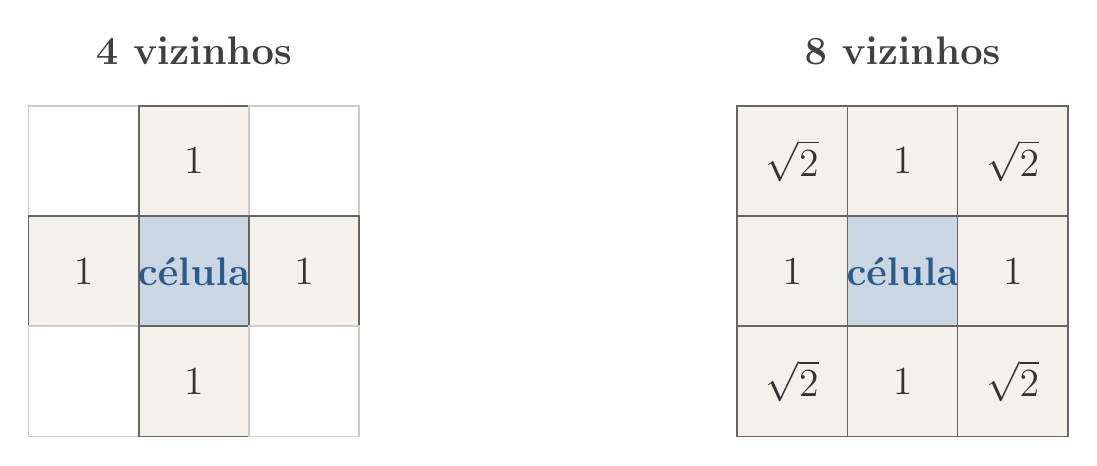
\begin{tikzpicture}[x=1cm,y=1cm]
\node[font=\Large\bfseries, black!75] at (2.10,4.9) {4 vizinhos};
\draw[fill=white, draw=black!20, line width=0.6pt] (0.00,2.80) rectangle ++(1.4,1.4);
\draw[fill=dcream, draw=black!60, line width=0.6pt] (1.40,2.80) rectangle ++(1.4,1.4);
\node[font=\Large, black!80] at (2.10,3.50) {1};
\draw[fill=white, draw=black!20, line width=0.6pt] (2.80,2.80) rectangle ++(1.4,1.4);
\draw[fill=dcream, draw=black!60, line width=0.6pt] (0.00,1.40) rectangle ++(1.4,1.4);
\node[font=\Large, black!80] at (0.70,2.10) {1};
\draw[fill=dblue!25!white, draw=black!60, line width=0.6pt] (1.40,1.40) rectangle ++(1.4,1.4);
\node[font=\Large\bfseries, dblue] at (2.10,2.10) {célula};
\draw[fill=dcream, draw=black!60, line width=0.6pt] (2.80,1.40) rectangle ++(1.4,1.4);
\node[font=\Large, black!80] at (3.50,2.10) {1};
\draw[fill=white, draw=black!20, line width=0.6pt] (0.00,0.00) rectangle ++(1.4,1.4);
\draw[fill=dcream, draw=black!60, line width=0.6pt] (1.40,0.00) rectangle ++(1.4,1.4);
\node[font=\Large, black!80] at (2.10,0.70) {1};
\draw[fill=white, draw=black!20, line width=0.6pt] (2.80,0.00) rectangle ++(1.4,1.4);
\node[font=\Large\bfseries, black!75] at (11.10,4.9) {8 vizinhos};
\draw[fill=dcream, draw=black!60, line width=0.6pt] (9.00,2.80) rectangle ++(1.4,1.4);
\node[font=\Large, black!80] at (9.70,3.50) {$\sqrt{2}$};
\draw[fill=dcream, draw=black!60, line width=0.6pt] (10.40,2.80) rectangle ++(1.4,1.4);
\node[font=\Large, black!80] at (11.10,3.50) {1};
\draw[fill=dcream, draw=black!60, line width=0.6pt] (11.80,2.80) rectangle ++(1.4,1.4);
\node[font=\Large, black!80] at (12.50,3.50) {$\sqrt{2}$};
\draw[fill=dcream, draw=black!60, line width=0.6pt] (9.00,1.40) rectangle ++(1.4,1.4);
\node[font=\Large, black!80] at (9.70,2.10) {1};
\draw[fill=dblue!25!white, draw=black!60, line width=0.6pt] (10.40,1.40) rectangle ++(1.4,1.4);
\node[font=\Large\bfseries, dblue] at (11.10,2.10) {célula};
\draw[fill=dcream, draw=black!60, line width=0.6pt] (11.80,1.40) rectangle ++(1.4,1.4);
\node[font=\Large, black!80] at (12.50,2.10) {1};
\draw[fill=dcream, draw=black!60, line width=0.6pt] (9.00,0.00) rectangle ++(1.4,1.4);
\node[font=\Large, black!80] at (9.70,0.70) {$\sqrt{2}$};
\draw[fill=dcream, draw=black!60, line width=0.6pt] (10.40,0.00) rectangle ++(1.4,1.4);
\node[font=\Large, black!80] at (11.10,0.70) {1};
\draw[fill=dcream, draw=black!60, line width=0.6pt] (11.80,0.00) rectangle ++(1.4,1.4);
\node[font=\Large, black!80] at (12.50,0.70) {$\sqrt{2}$};
\end{tikzpicture}
\end{document}
